%%%%%%%%%%%%%%%%%%%%%%%%%%%%%%%%%%%%%%%%%%%%%%%%%%%%%%%%%%%%
%%% ELIFE ARTICLE TEMPLATE
%%%%%%%%%%%%%%%%%%%%%%%%%%%%%%%%%%%%%%%%%%%%%%%%%%%%%%%%%%%%
%%% PREAMBLE 
\documentclass[9pt,lineno]{elife}
% Use the onehalfspacing option for 1.5 line spacing
% Use the doublespacing option for 2.0 line spacing
% Please note that these options may affect formatting.

\usepackage{lipsum} % Required to insert dummy text
\usepackage[version=4]{mhchem}
\usepackage{siunitx}
\DeclareSIUnit\Molar{M}

\usepackage{float}
\newfloat{suppfile}{thp}{lofsupfile}
\floatname{suppfile}{Supplementary file}

\usepackage{placeins}

\renewcommand{\floatpagefraction}{1}

\newcommand{\jdbcomment}[1]{\emph{\color{red} [#1]}}

%%%%%%%%%%%%%%%%%%%%%%%%%%%%%%%%%%%%%%%%%%%%%%%%%%%%%%%%%%%%
%%% ARTICLE SETUP
%%%%%%%%%%%%%%%%%%%%%%%%%%%%%%%%%%%%%%%%%%%%%%%%%%%%%%%%%%%%
\title{Shifting mutational effects on the evolutionary landscape of HIV Envelope}

\author[1,2\authfn{1}]{Hugh K. Haddox}
\author[1,2\authfn{1}]{Adam S. Dingens}
\author[1,3]{Sarah K. Hilton}
\author[4]{Julie Overbaugh}
\author[1,2,3]{Jesse D. Bloom}
\affil[1]{Basic Sciences Division and Computational Biology Program, Fred Hutchinson Cancer Research Center, Seattle, WA}
\affil[2]{Molecular and Cellular Biology PhD program, University of Washington, Seattle, WA}
\affil[3]{Department of Genome Sciences, University of Washington, Seattle, WA}
\affil[4]{Human Biology Division, Fred Hutchinson Cancer Research Center, Seattle, WA}
\contrib[\authfn{1}]{These authors contributed equally to this work}

\corr{jbloom@fredhutch.org}{JDB}
% \presentadd[\authfn{5}]{eLife Sciences editorial Office, eLife Sciences, Cambridge, United Kingdom}

%%%%%%%%%%%%%%%%%%%%%%%%%%%%%%%%%%%%%%%%%%%%%%%%%%%%%%%%%%%%
%%% ARTICLE START
%%%%%%%%%%%%%%%%%%%%%%%%%%%%%%%%%%%%%%%%%%%%%%%%%%%%%%%%%%%%

\begin{document}

\maketitle

\begin{abstract}
HIV Envelope (Env) evolves rapidly.
The immediate the evolutionary space accessible to any viral variant is largely determined by the effects of single amino-acid mutations.
However, the effects of these mutations can shift over evolutionary time as the virus traverses through sequence space.
Here we comprehensively quantify the ways in which mutational effects shift or remain constant by experimentally measuring the effects of all amino-acid mutations to two homologs of Env with 85\% (?) sequence identity.
We find...
\end{abstract}


\section{Introduction}


\section{Results}

\subsection*{Deep mutational scanning of two Env homologs from transmitted-founder (?) viruses}

\begin{figure}
\centerline{\bf \Large A \hspace{0.52\textwidth} \bf B \hspace{0.35\textwidth}}
\centerline{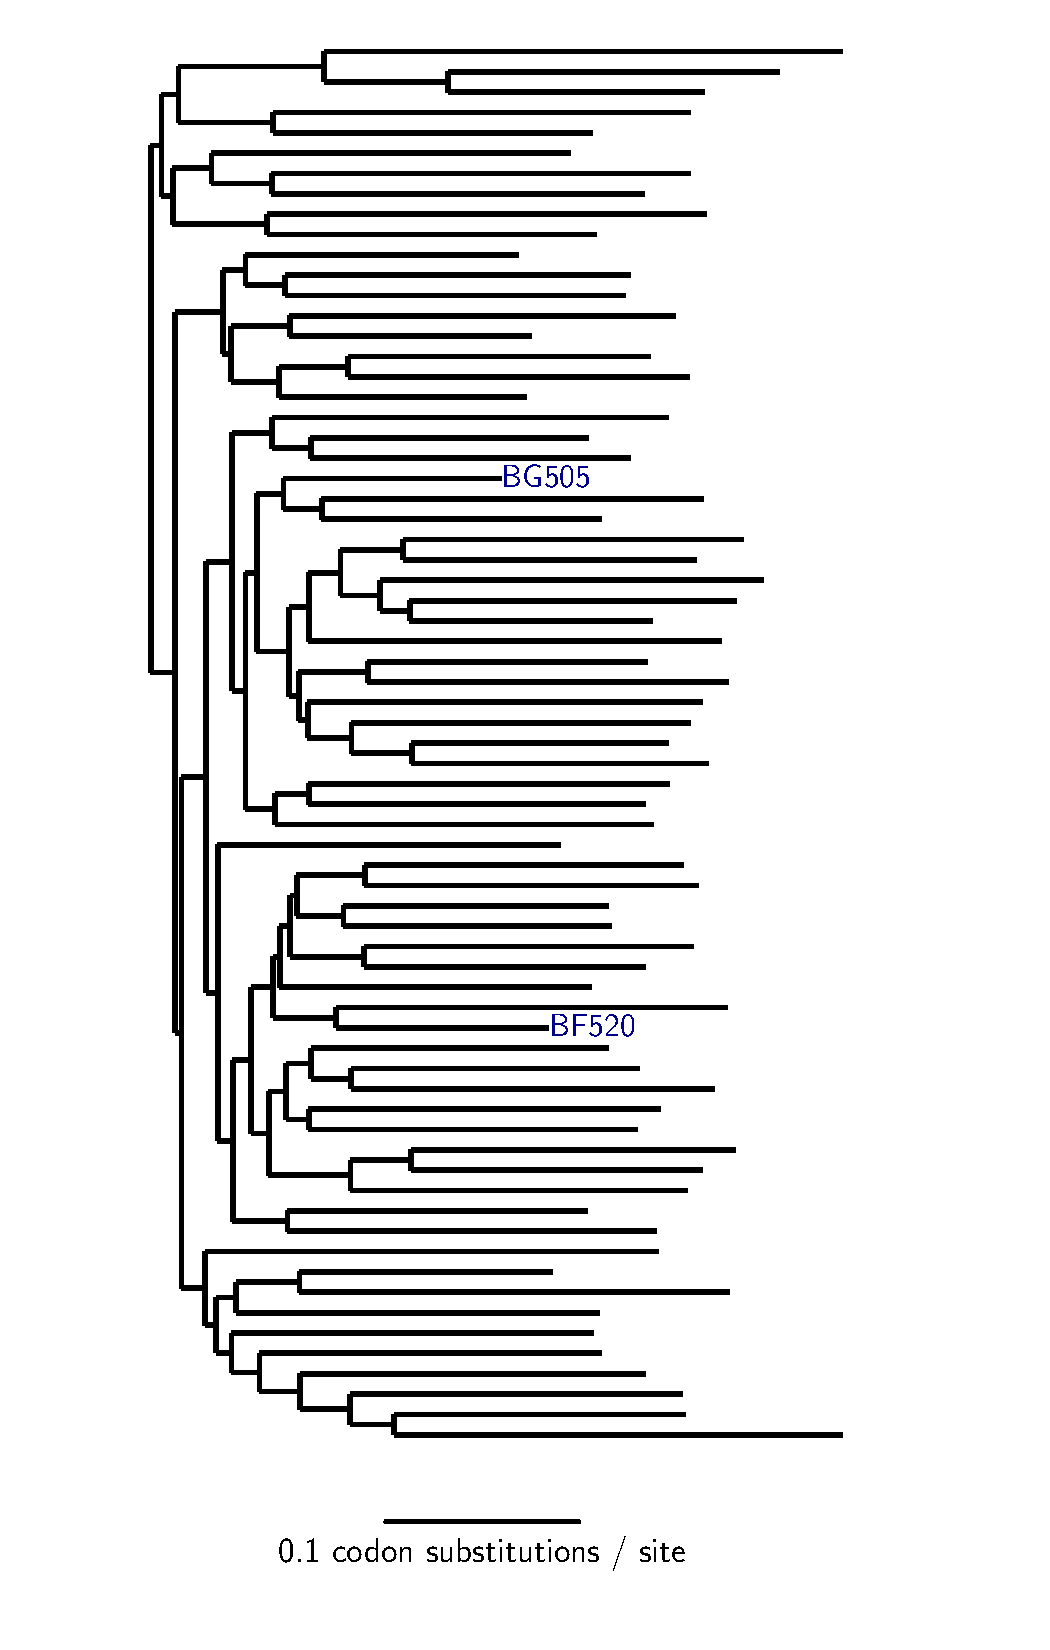
\includegraphics[width=0.64\textwidth]{figures/tree_plot.pdf} 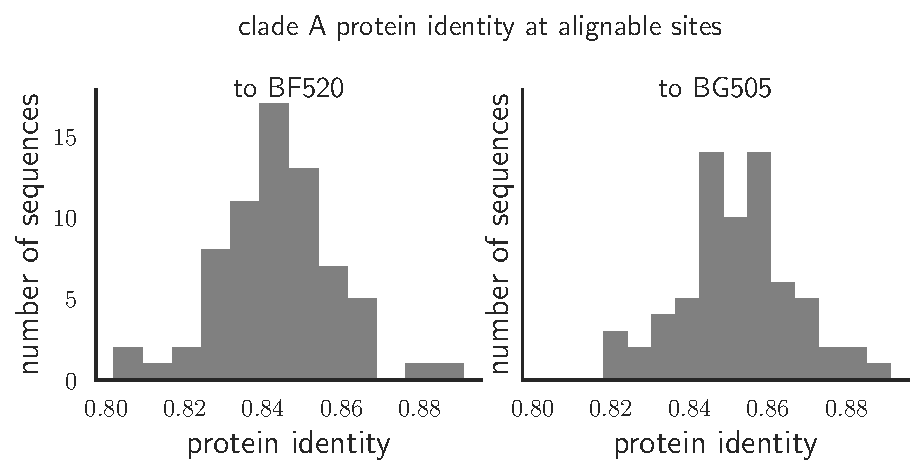
\includegraphics[width=0.36\textwidth]{figures/masked_alignment_identity.pdf}}
\caption{\label{fig:tree}
CAPTION
}
\figdata{The coding sequence alignment of clade A \textit{env} sequences in FASTA format is in \texttt{cladeA\_alignment.fasta}.}
\figdata{Sites masked in all phylogenetic analyses because they were not mutagenized in our experiments or are poorly alignable are listed in \texttt{alignment\_mask.csv}.}
\end{figure}
\FloatBarrier

\begin{figure}
\centerline{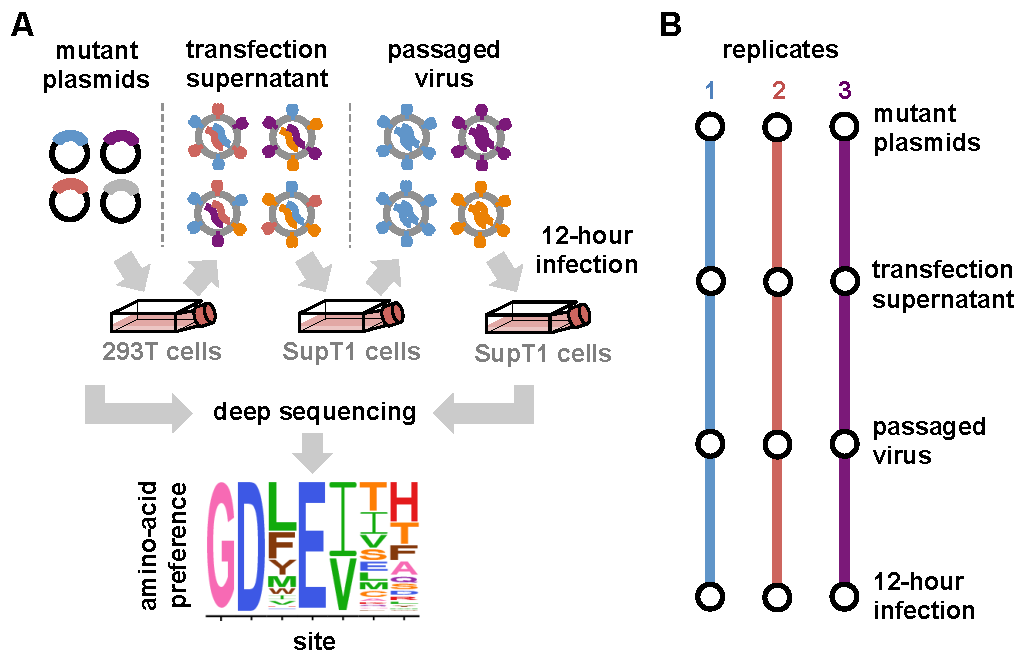
\includegraphics[width=0.85\textwidth]{figures/dms_schematic/dms_schematic.pdf}}
\caption{\label{fig:dms_schematic}
Deep mutational scanning workflow.
{\bf (A)} For each homolog, we made a library of proviral HIV plasmids with random codon-level mutations in \textit{env}.
We then transfected the plasmids into 293T cells to generate mutant viruses, which may lack a genotype-phenotype link since transfected cell are expected to each receive multiple plasmids.
To establish this link and select for functional variants, we first passaged the libraries in SupT1 cells at a low MOI.
Then, we imposed a second round of selection by infecting the passaged viruses into SupT1 cells at a high MOI and then harvesting reverse-transcribed unintegrated viral DNA at 12 hours post-infection.
Finally, we deep sequenced the libraries before and after selection.
We also deep sequenced wildtype controls to estimate error rates due to PCR, deep sequencing, and viral replication.
Using these sequencing data, we then inferred each site's preference for each of the 20 amino acids.
{\bf (B)} For each homolog, we conducted this experiment in full biological triplicate, beginning at the stage of independently creating the plasmid mutant libraries.
}
\figsupp[Sanger sequencing of the BG505 mutant plasmid libraries.]{
We Sanger sequenced 44 clones of BG505 Env sampled roughly evenly from each of the three replicate mutant plasmid libraries.
{\bf(A)} There was an average of 1.5 mutant codons per clone, with the number of mutations per clone roughly following a Poisson distribution. 
{\bf(B)} The mutant codons had a mix of single-, double-, and triple-nucleotide changes, with an elevated number of single-nucleotide changes than expected.
{\bf(C)} Nucleotide frequencies were fairly uniform in the mutant codons.
{\bf(D)} Mutations were distributed roughly evenly along the mutagenized region of {\it env} (30-699 in the sequential numbering scheme used here).
{\bf(E)} For clones with multiple mutations, we computed the pairwise distance in primary sequence between each codon mutation and plotted the cumulative distribution of these distances (red line). 
We also simulated the expected distribution of pairwise distances if mutations occurred entirely independently (blue line). 
The observed distribution is close to the expected distribution.
}{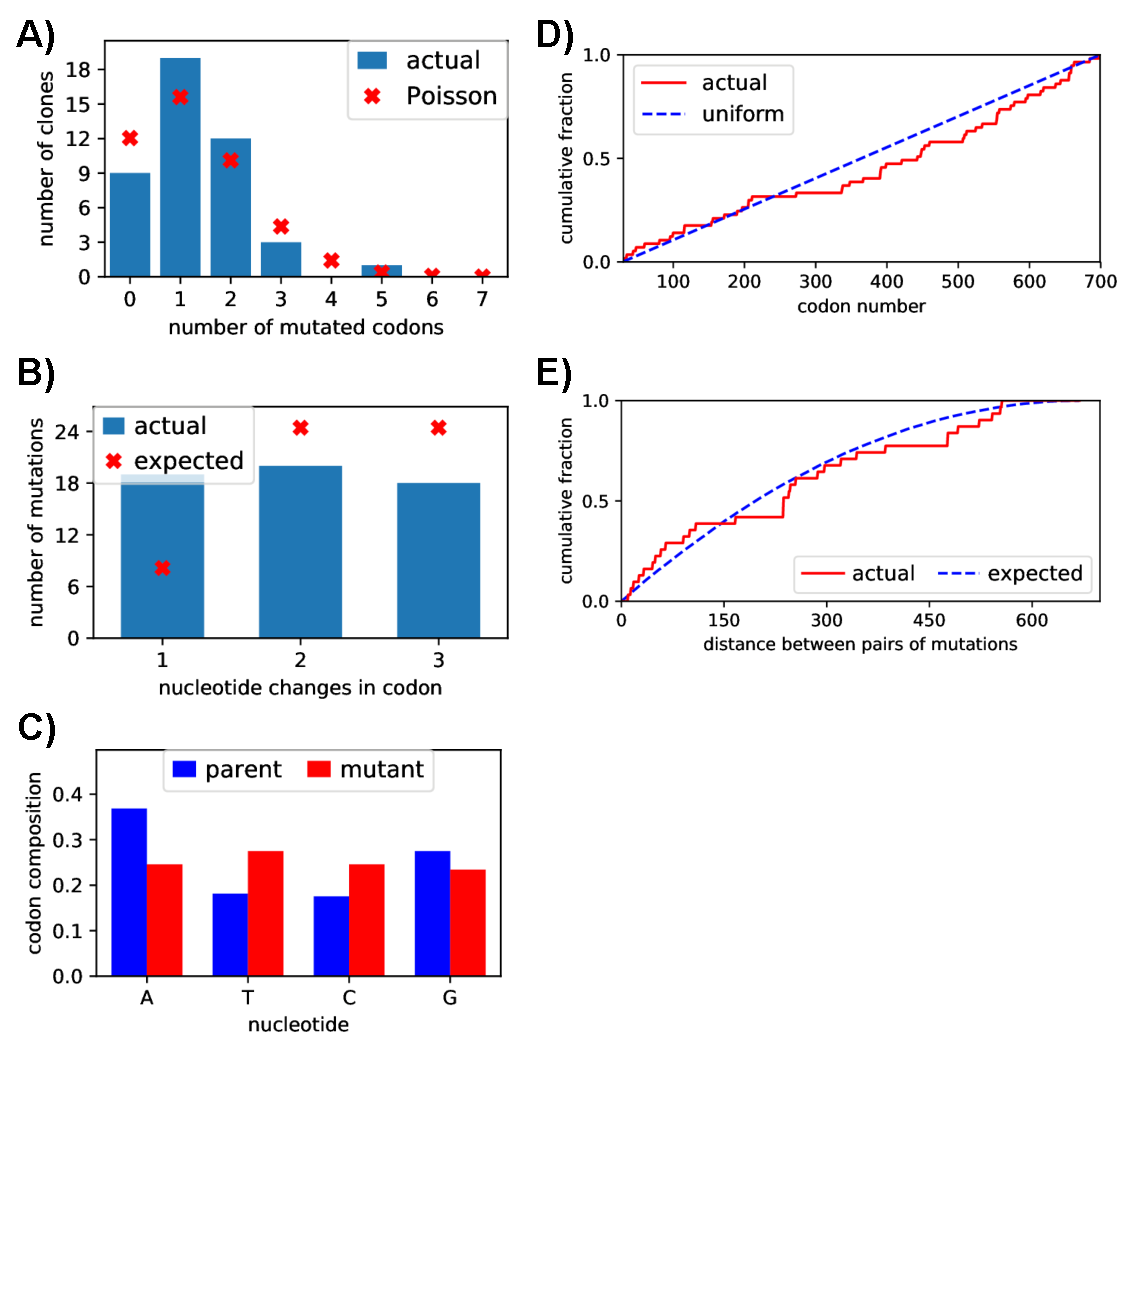
\includegraphics[width=\textwidth]{figures/sanger_sequencing_supp/sanger_sequencing_supp.pdf}}
\end{figure}
\FloatBarrier

\begin{figure}
%{{\bf \Large A} \hspace{0.2\textwidth} BG505 \hspace{0.51\textwidth} BF520} \\
%{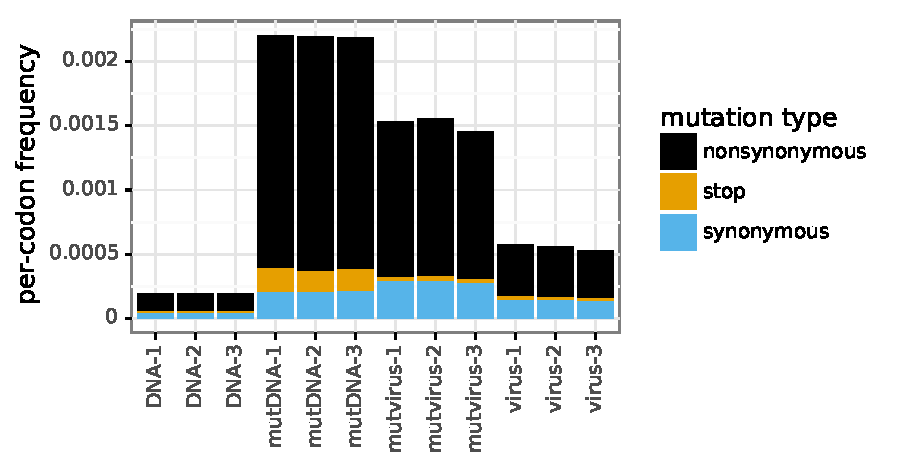
\includegraphics[height=0.32\textwidth]{figures/BG505_avgmutfreqs.pdf}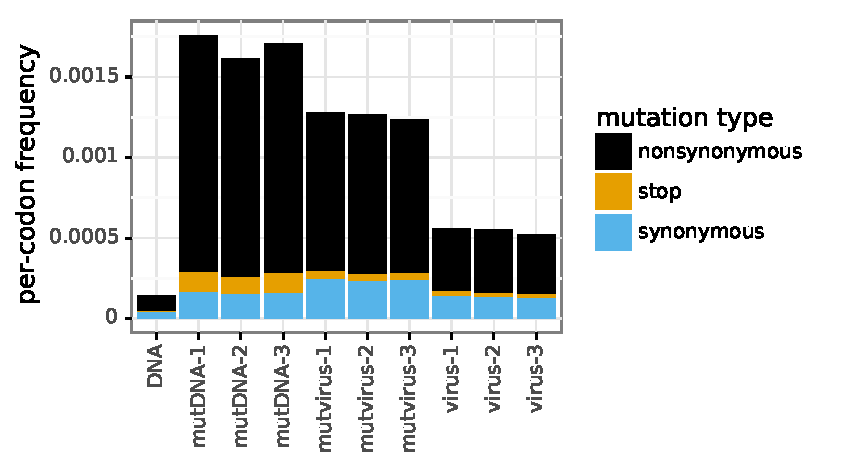
\includegraphics[clip=true,trim=0in 0in 1.7in 0in,height=0.32\textwidth]{figures/BF520_avgmutfreqs.pdf}} \\
%{\bf \Large B} \\
%{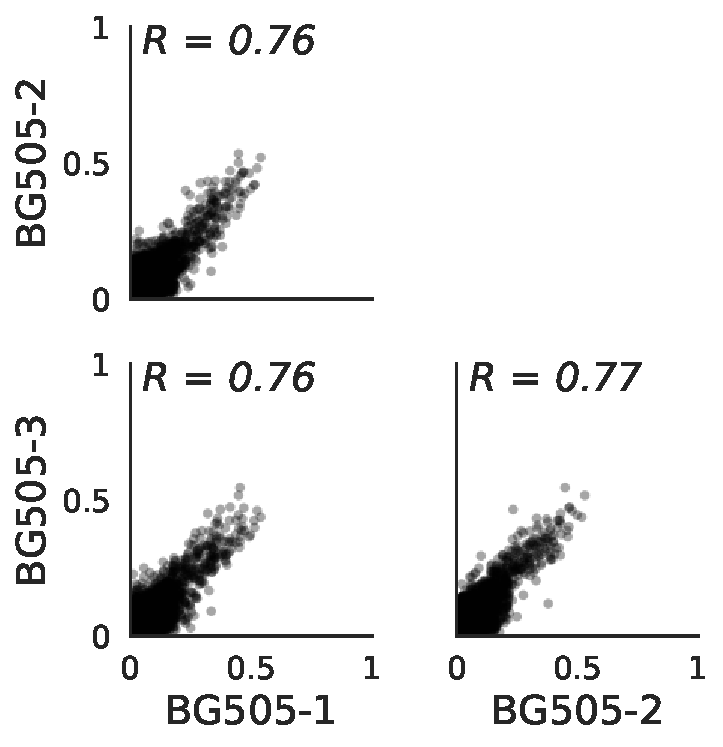
\includegraphics[width=0.37\textwidth]{figures/BG505_prefscorr.pdf}\hspace{0.1\textwidth}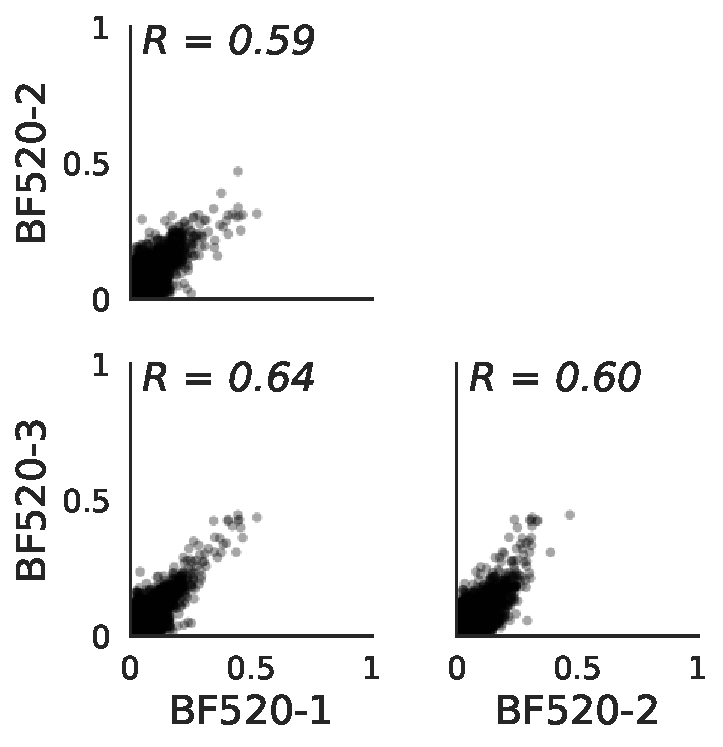
\includegraphics[width=0.37\textwidth]{figures/BF520_prefscorr.pdf}}
\begin{minipage}[t]{0.34\textwidth}
{\bf \Large A} \\ 
\centerline{{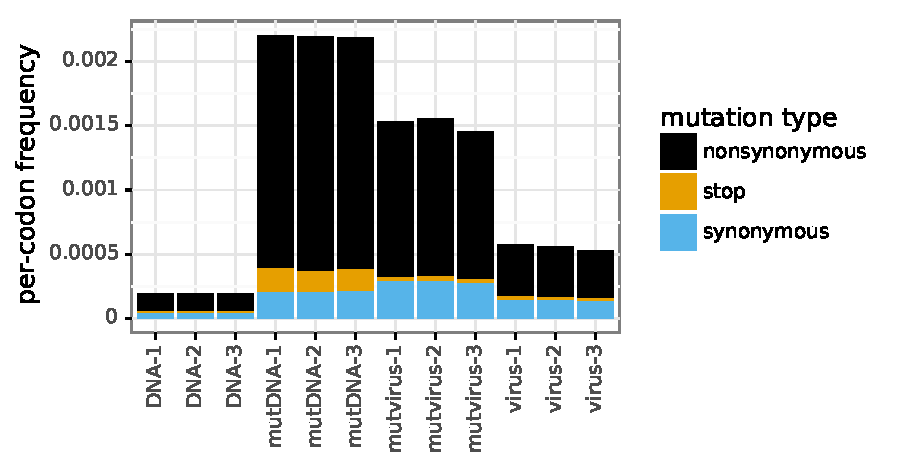
\includegraphics[clip=true, trim=4.3in 1.4in 0in 0.48in, width=0.4\textwidth]{figures/BG505_avgmutfreqs.pdf}}} 
\centerline{\small BG505}
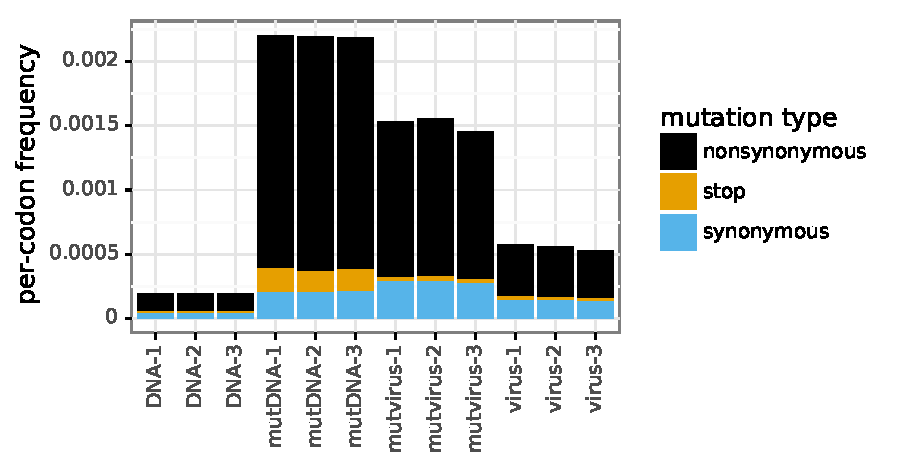
\includegraphics[clip=true, trim=0in 0in 1.7in 0in, width=\textwidth]{figures/BG505_avgmutfreqs.pdf}
\centerline{\small BF520}
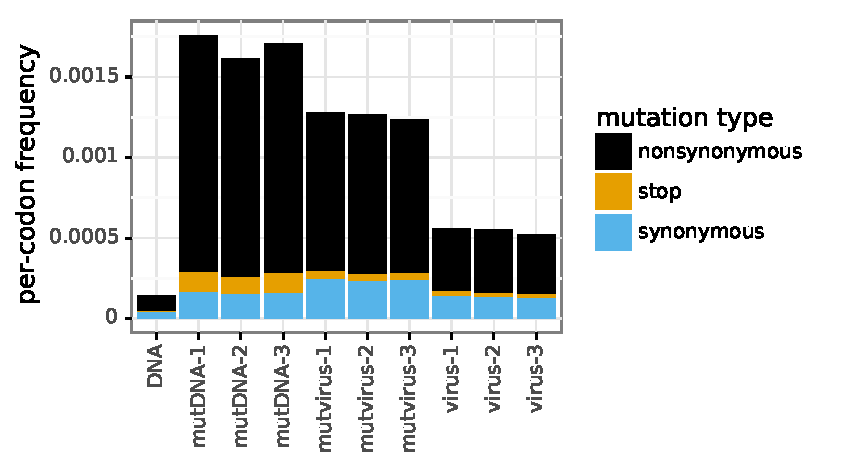
\includegraphics[clip=true, trim=0in 0in 1.7in 0in, width=0.89\textwidth]{figures/BF520_avgmutfreqs.pdf}
\end{minipage}
\begin{minipage}[t]{0.01\textwidth}
\end{minipage}
\begin{minipage}[t]{0.65\textwidth}
{\bf \Large B} \\
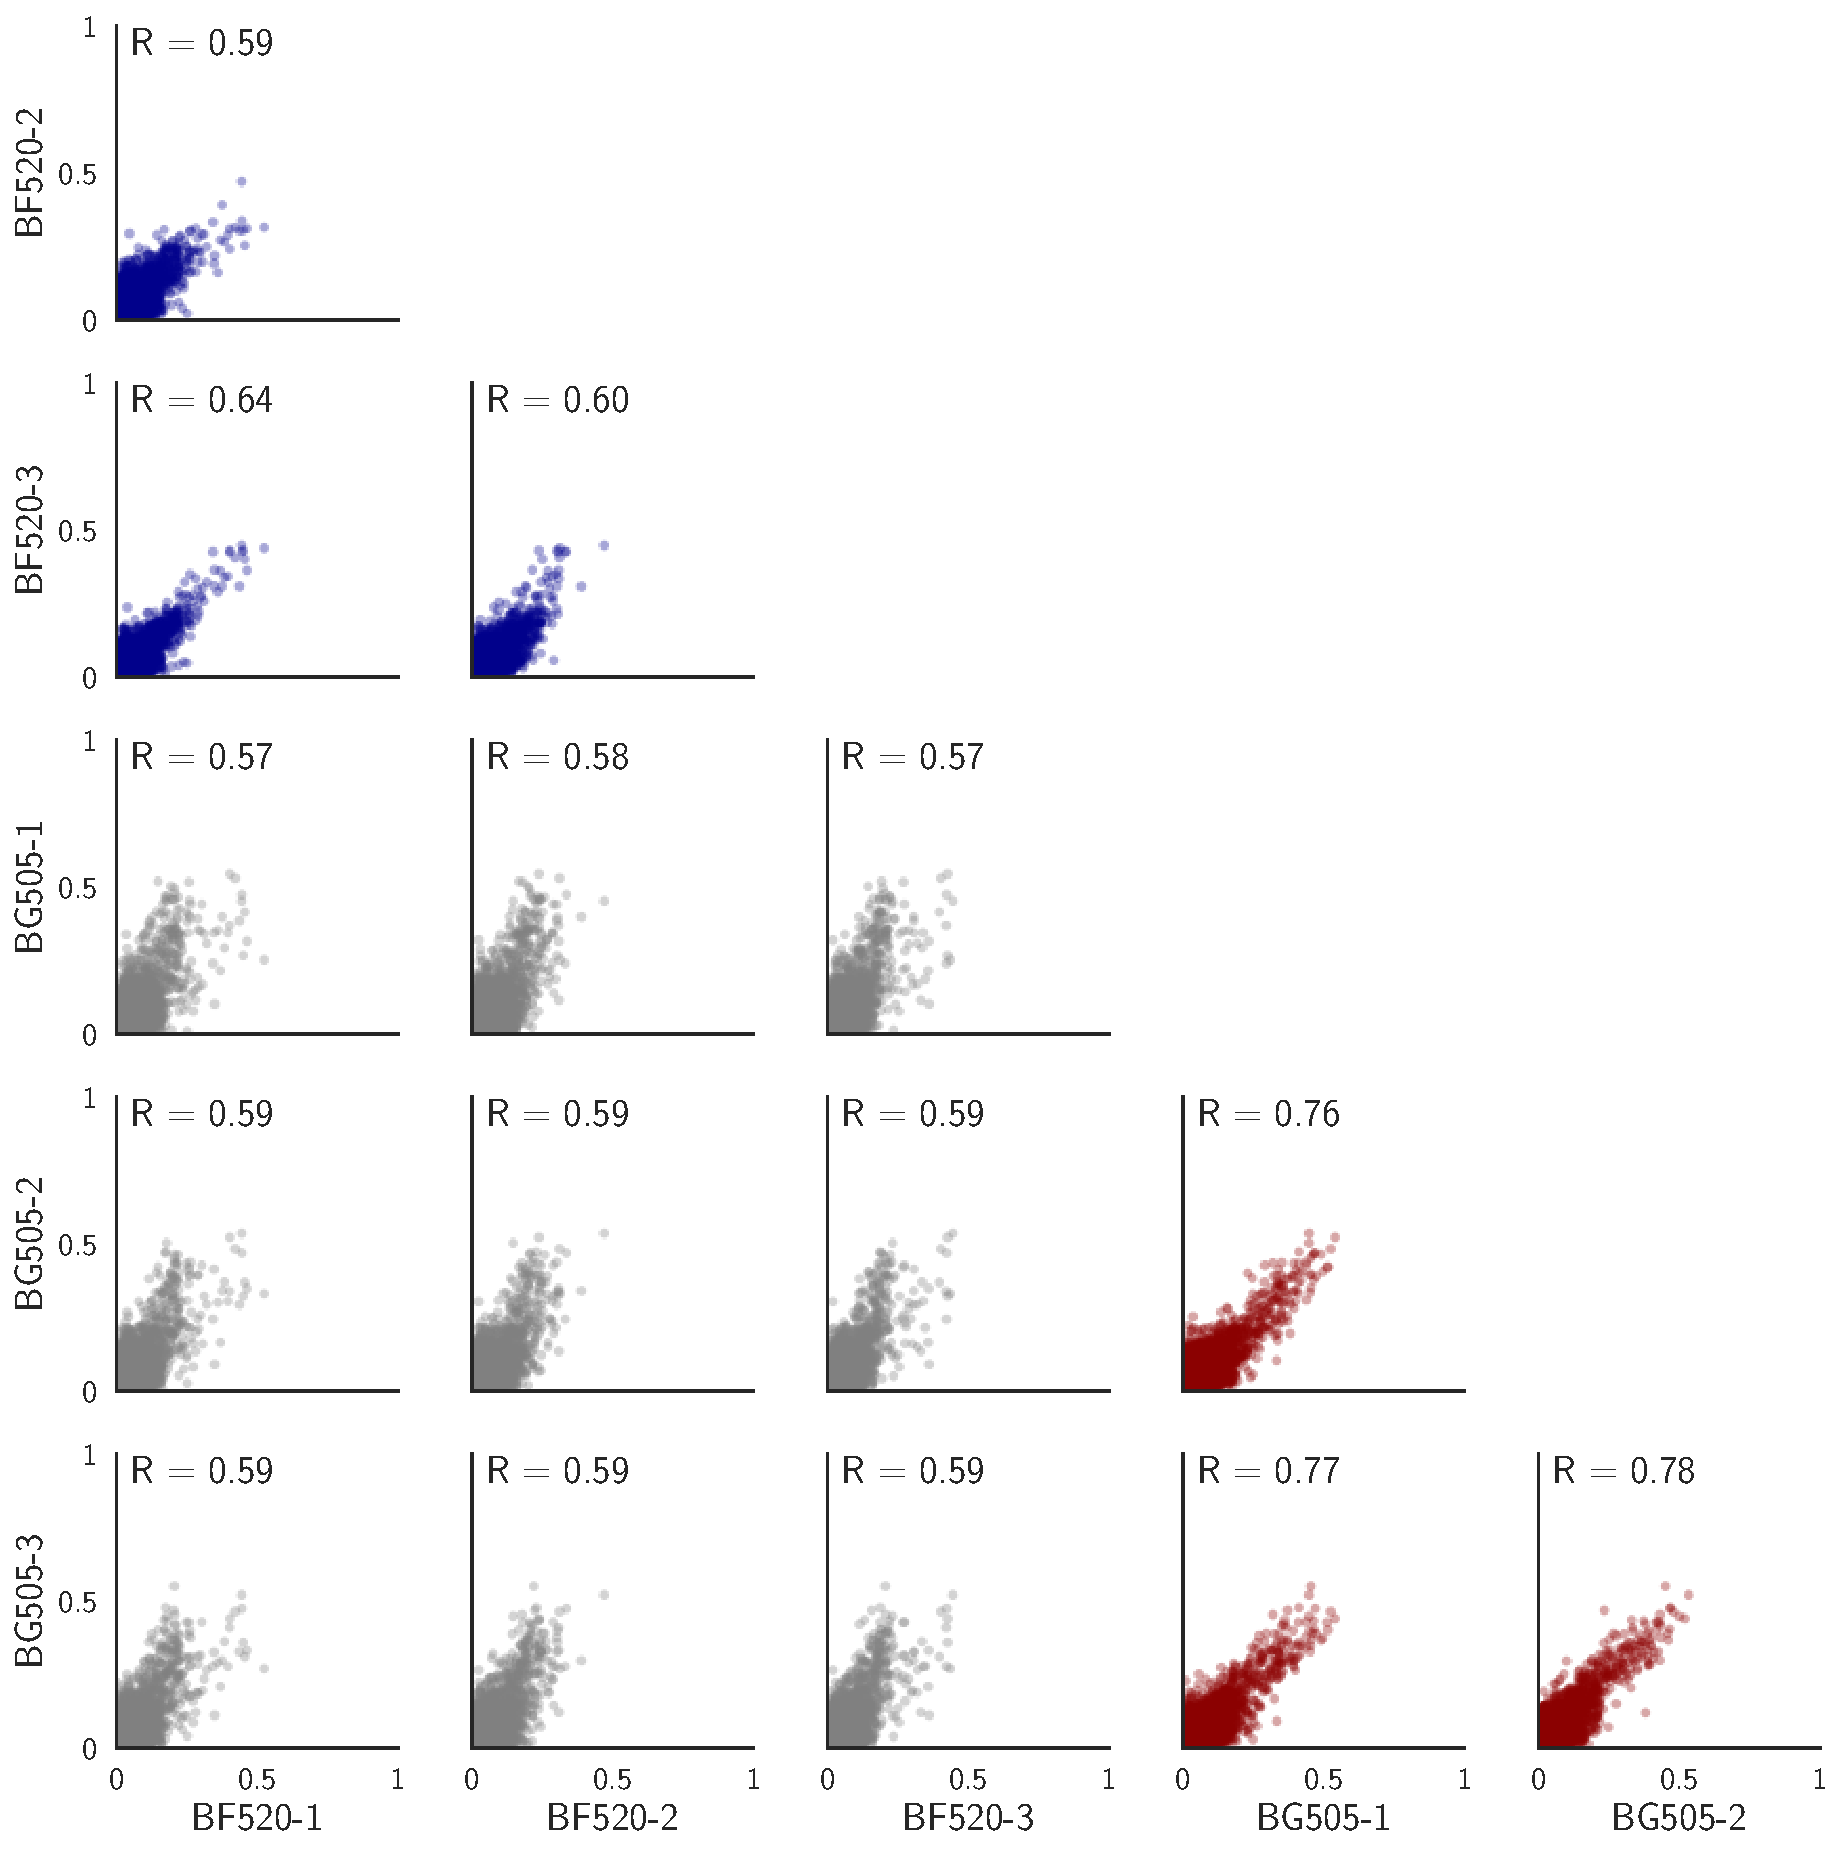
\includegraphics[width=\textwidth]{figures/allprefscorr.pdf}
\end{minipage}
\caption{\label{fig:mutfreqs}
CAPTION
}
\figdata{The raw numerical data plotted in panel (A) are in the file \texttt{avgmutfreqs.csv}.}
\figdata{The amino-acid preferences for each replicate and the replicate averages for each homolog are in \texttt{all\_prefs\_unscaled.zip}.}
\end{figure}
\FloatBarrier



\subsection*{Re-scaling the experimental measurements to optimally describe HIV evolution in nature}

\begin{table}
\begin{fullwidth}
{\centering \begin{tabular}{lrrrrrrrrr}
\toprule
           Model &  $\Delta$AIC &  LogLikelihood &  nParams &  stringency &  $\overline{\omega}$ &  $\omega_{\alpha}$ &  $\omega_{\beta}$ &  nsites $\omega_r > 1$ &  nsites $\omega_r < 1$ \\
\midrule
     ExpCM BF520 &          0.0 &       -35218.8 &        7 &         2.8 &                  1.4 &                1.0 &               0.7 &                     66 &                     35 \\
     ExpCM BG505 &        269.0 &       -35353.3 &        7 &         2.1 &                  1.3 &                0.9 &               0.7 &                     65 &                     53 \\
 Goldman-Yang M5 &       3455.1 &       -36941.4 &       12 &         nan &                  0.8 &                0.6 &               0.7 &                     14 &                    211 \\
\bottomrule
\end{tabular}
}
\caption{\label{tab:phydms}
Phylogenetic models that incorporate Env's preferences indicate that selection was less stringent in the lab than in nature.}
\tabledata{Results for phylogenetic models where $\omega$ is not drawn from a gamma-distribution or where the preferences are averaged across sites are in \texttt{modelcomparison.md}.}
\end{fullwidth}
\end{table}
\FloatBarrier

\begin{figure}
\begin{fullwidth}
{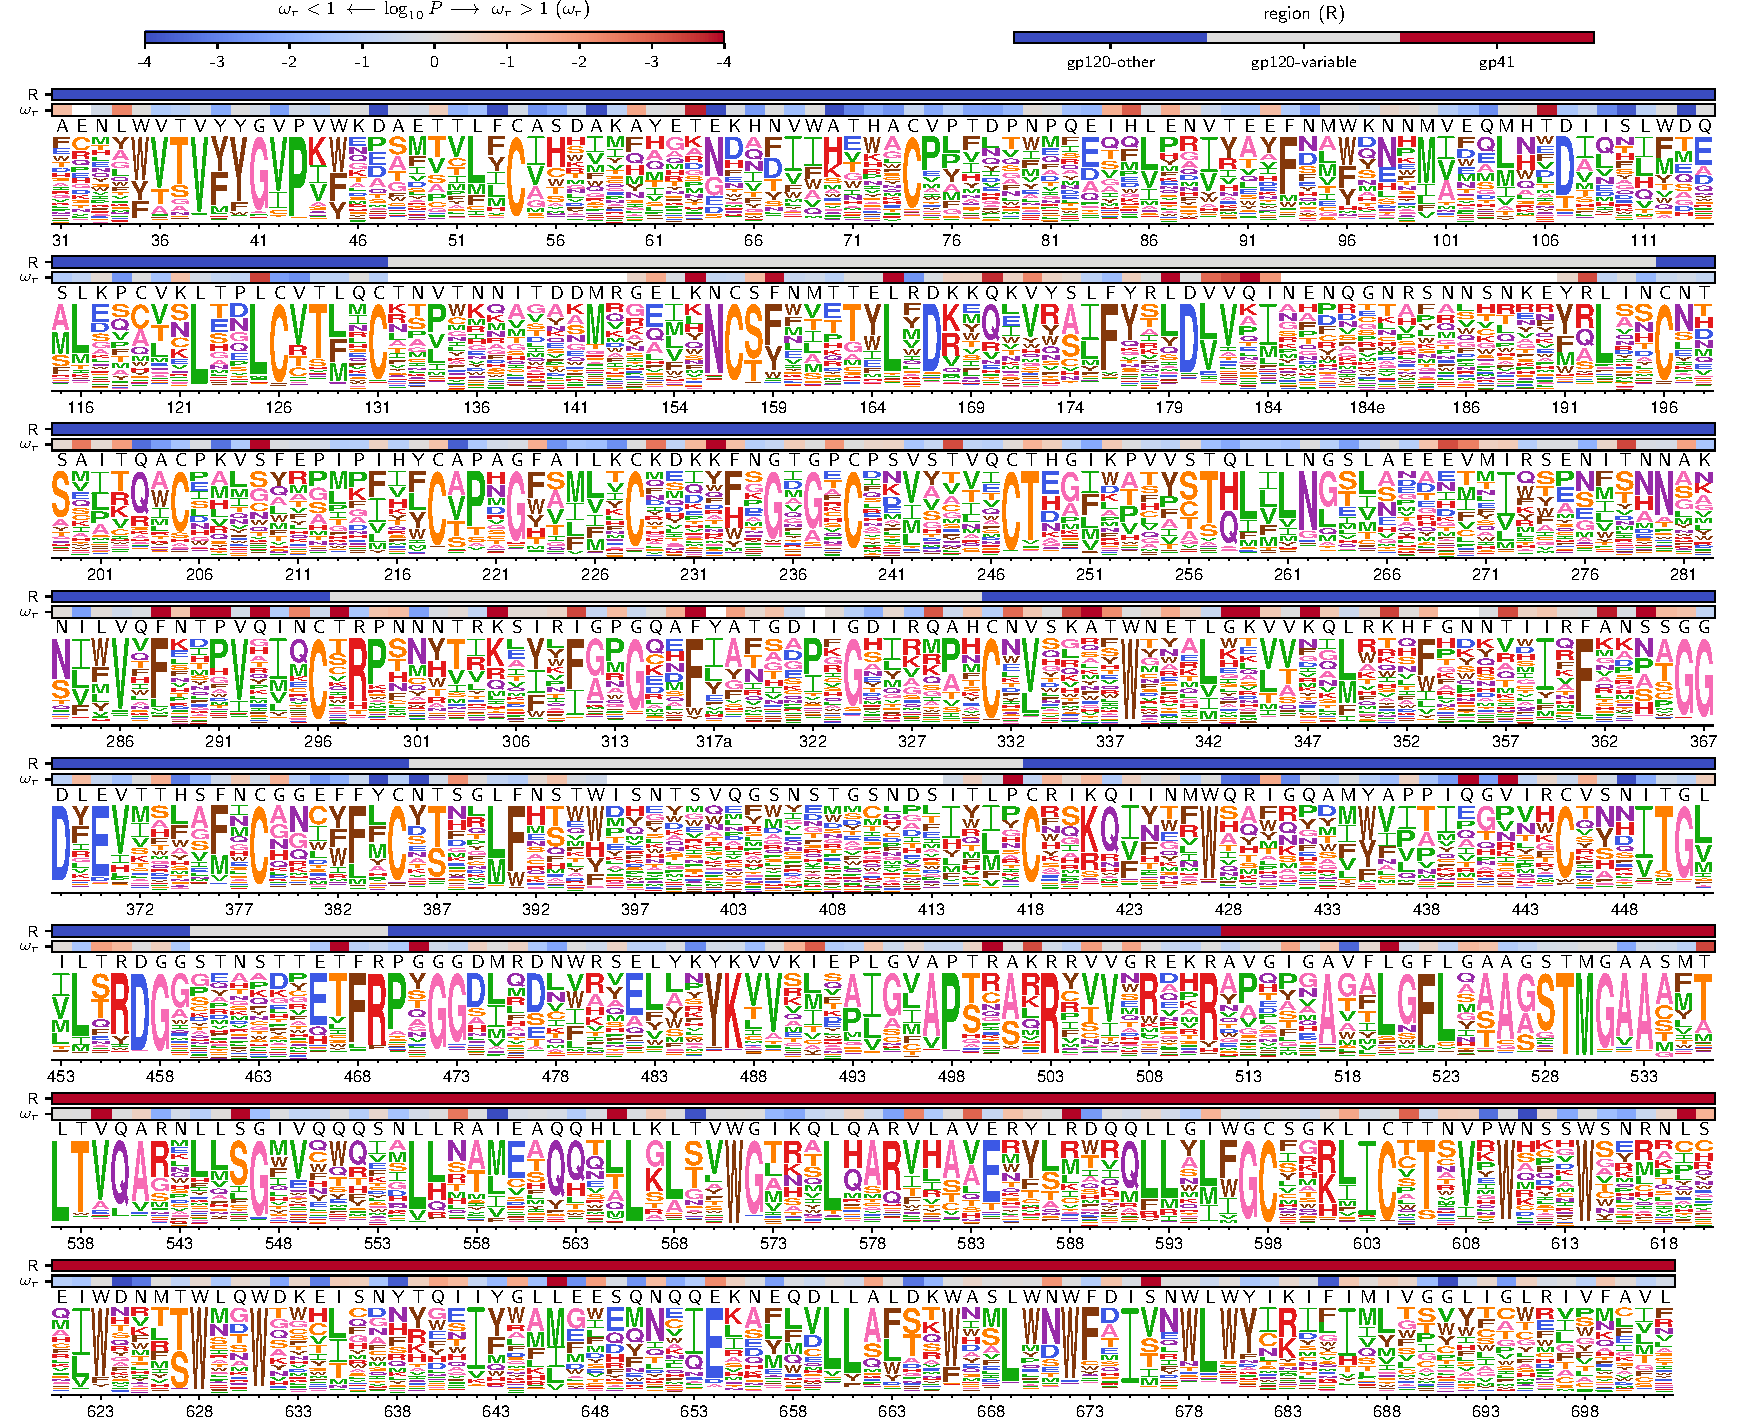
\includegraphics[width=1.3\textwidth]{figures/BG505_prefs.pdf}}
\caption{\label{fig:bg505_prefs_logo}
The rescaled averaged site-specific amino-acid preferences for BG505.
This logo plot shows the site-specific amino-acid preferences for BG505 after averaging between replicates and then rescaling them using the stringency parameter from Table \ref{tab:phydms} inferred for BG505 from the group-M alignment.
Each site has a stack of 20 letters corresponding to the 20 amino acids.
Letter heights, which sum to one at each site, are proportional to the site's preference for each amino acid.
The top bar (R) indicates gp120 variable loops, other regions in gp120, or gp41.
The bottom bar (WT) shows the wildtype amino-acid sequence for BG505.
Sites are numbered according to the HXB2 numbering scheme~\cite{korber1998numbering}).
}
\figdata{The re-scaled preferences plotted in this figure are in \texttt{rescaled\_BG505\_prefs.csv.}}
\figdata{Sequence of the BG505 Env and mapping from sequential 1, 2, ... numbering of this sequence (\emph{original} column) to HXB2 numbering (\emph{new} column) is in \texttt{BG505\_to\_HXB2.csv}.}
\figdata{The $\omega_r$ values and associated $P$-values for BG505 in HXB2 numbering are in \texttt{BG505\_omegabysite.tsv}.}
\end{fullwidth}
\end{figure}
\FloatBarrier

\begin{figure}
\begin{fullwidth}
{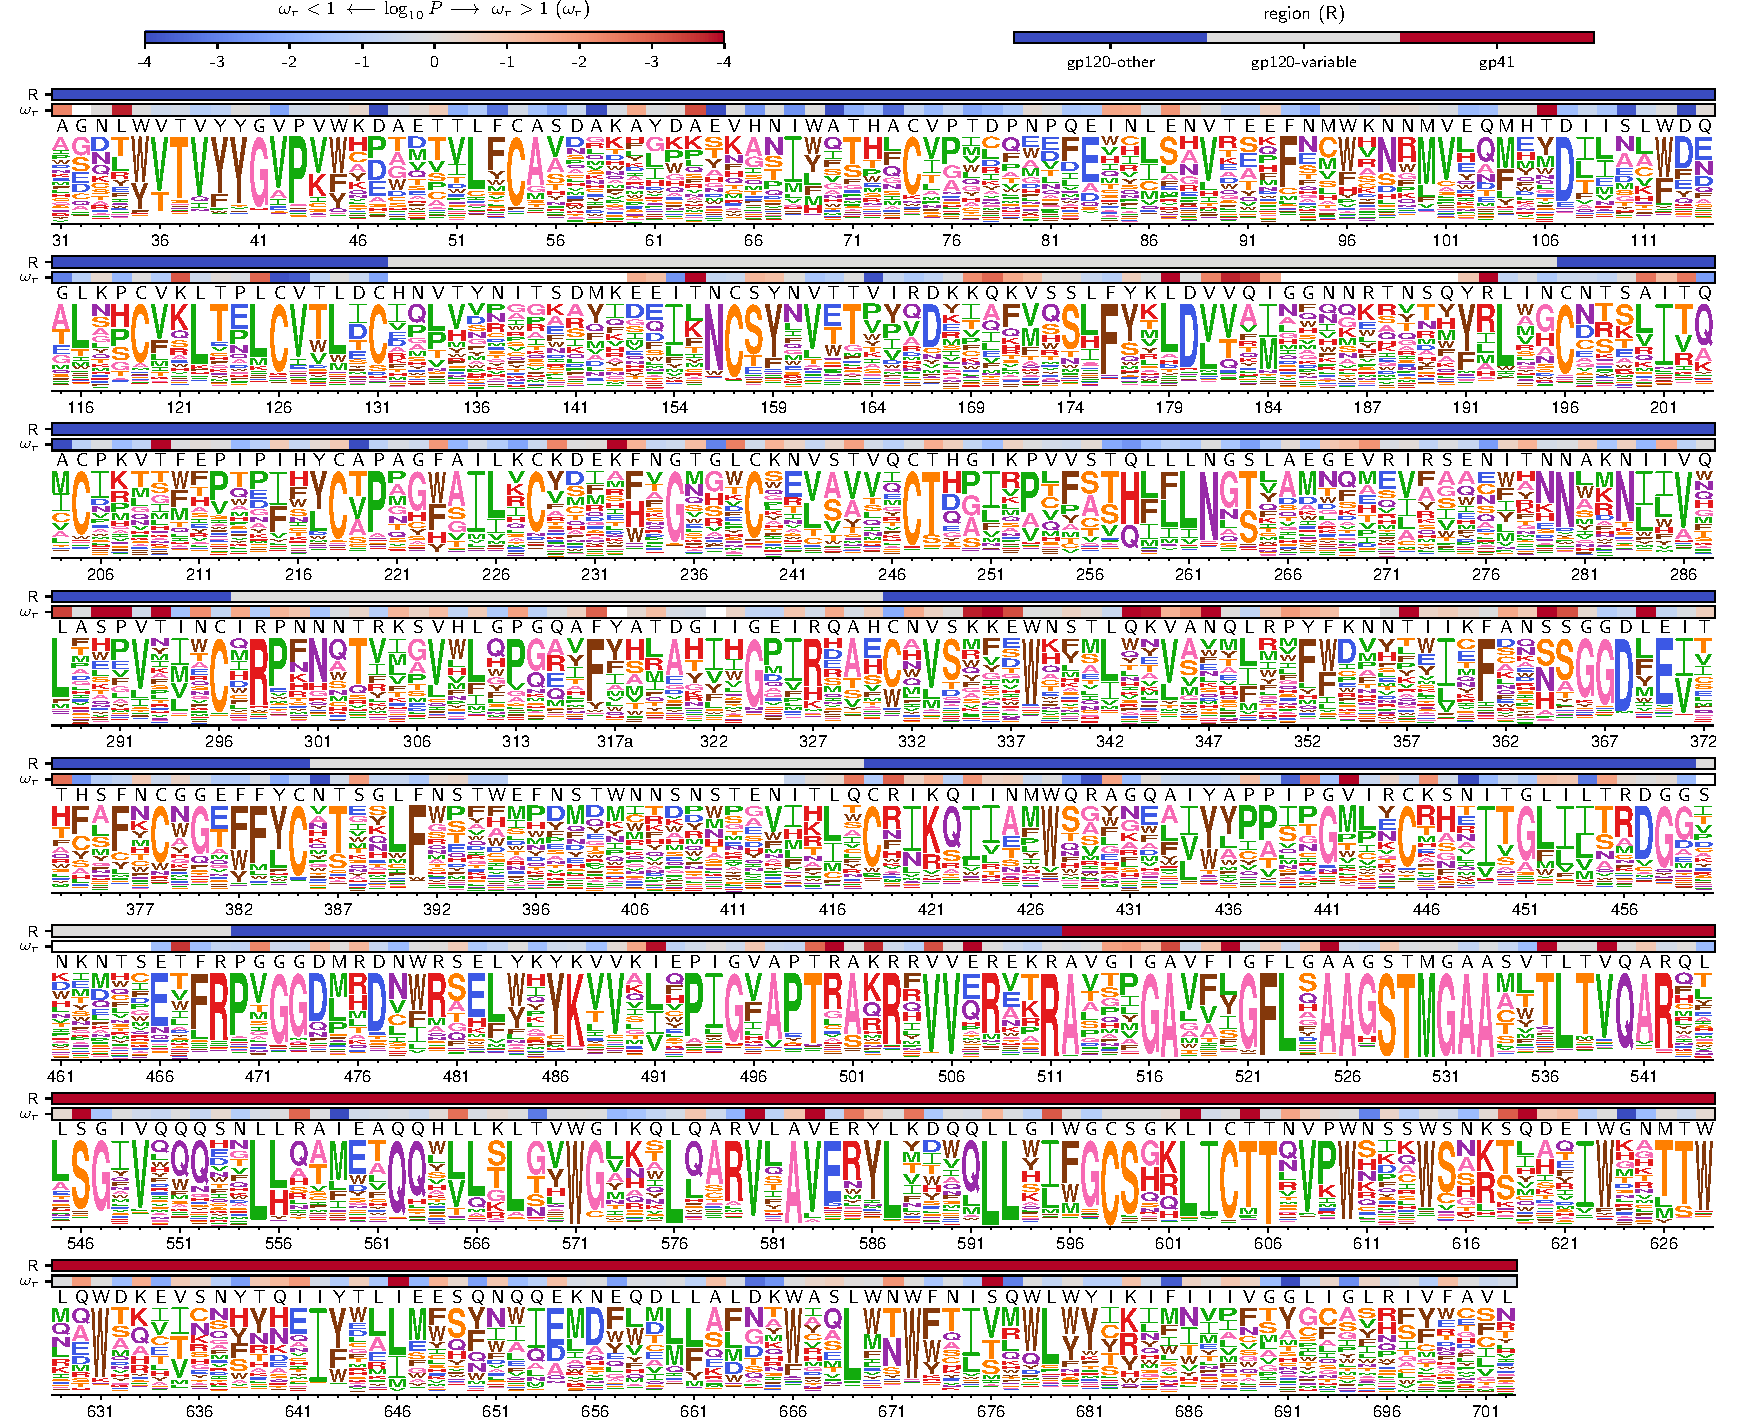
\includegraphics[width=1.3\textwidth]{figures/BF520_prefs.pdf}}
\caption{\label{fig:bf520_prefs_logo}
The re-scaled averaged site-specific amino-acid preferences for BF520.
This figure is the same as Fig \ref{fig:bg505_prefs_logo}, but for BF520 instead of BG505.
}
\figdata{The re-scaled preferences plotted in this figure are in \texttt{rescaled\_BF520\_prefs.csv.}}
\figdata{Sequence of the BF520 Env and mapping from sequential 1, 2, ... numbering of this sequence (\emph{original} column) to HXB2 numbering (\emph{new} column) is in \texttt{BF520\_to\_HXB2.csv}.}
\figdata{The $\omega_r$ values and associated $P$-values for BF520 in HXB2 numbering are in \texttt{BG505\_omegabysite.tsv}.}
\end{fullwidth}
\end{figure}
\FloatBarrier

\begin{figure}
%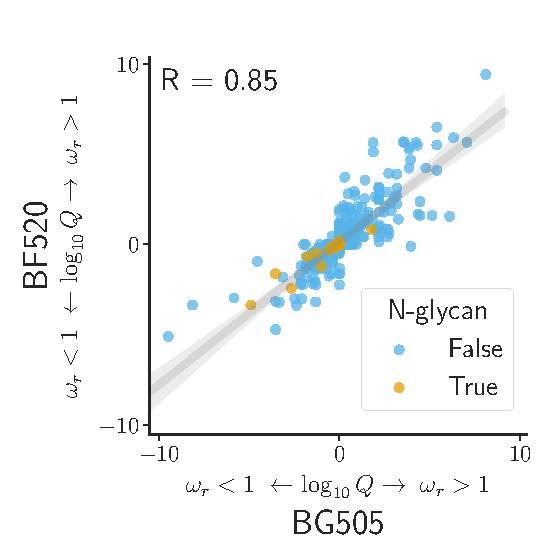
\includegraphics[width=0.5\textwidth]{figures/diversifying_selection_corr.pdf}
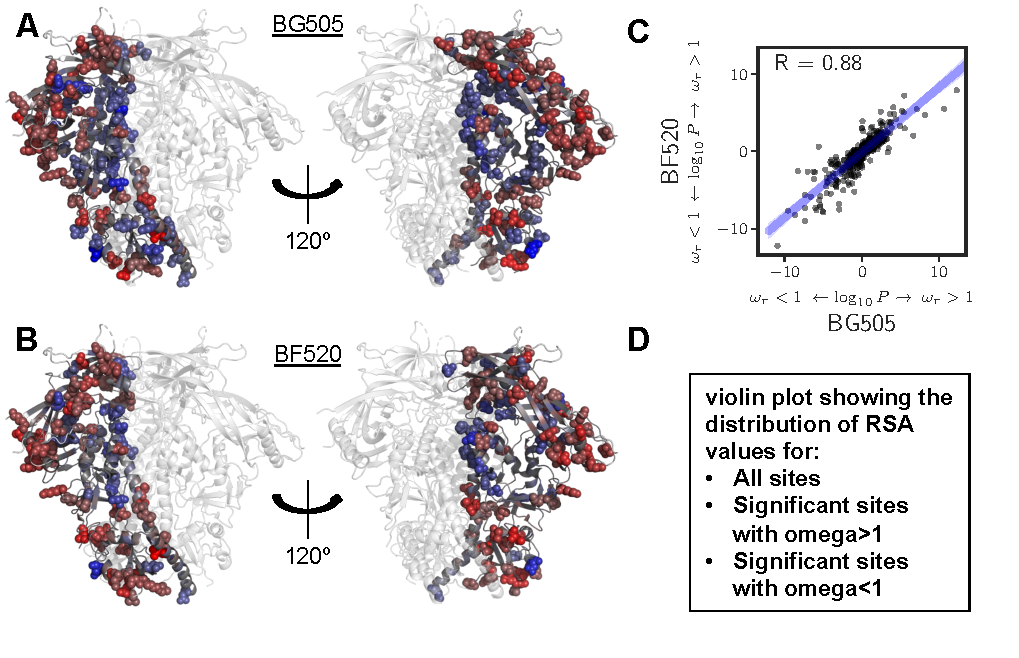
\includegraphics[width=1.0\textwidth]{figures/omegabysite_structural_analysis/omegabysite_structural_analysis.pdf}
\caption{\label{fig:divselcorr}
Correlation between sites of diversifying and purifying selection among homologs.
\jdbcomment{Hugh - can you make the panel showing the relationship between purifying selection and the Andrew Ward sites.}  
}
\figsupp[Amino-acid preferences and alignment frequencies at sites of purifying selection.]{
This plot shows all sites that are evolving more slowly than expected in natural sequences given the preferences measured in both homologs.
Specifically, it shows all sites with $\omega_r < 1$ at $Q < 0.05$ for the ExpCMs for \emph{both} BG505 and BF520.
For each site, the plots show the preferences averaged across replicates and re-scaled for each homolog, as well as the frequencies of amino acids in the clade A Env alignment. 
The $Q$-value indicated is the maximum of that for the two homologs.
}{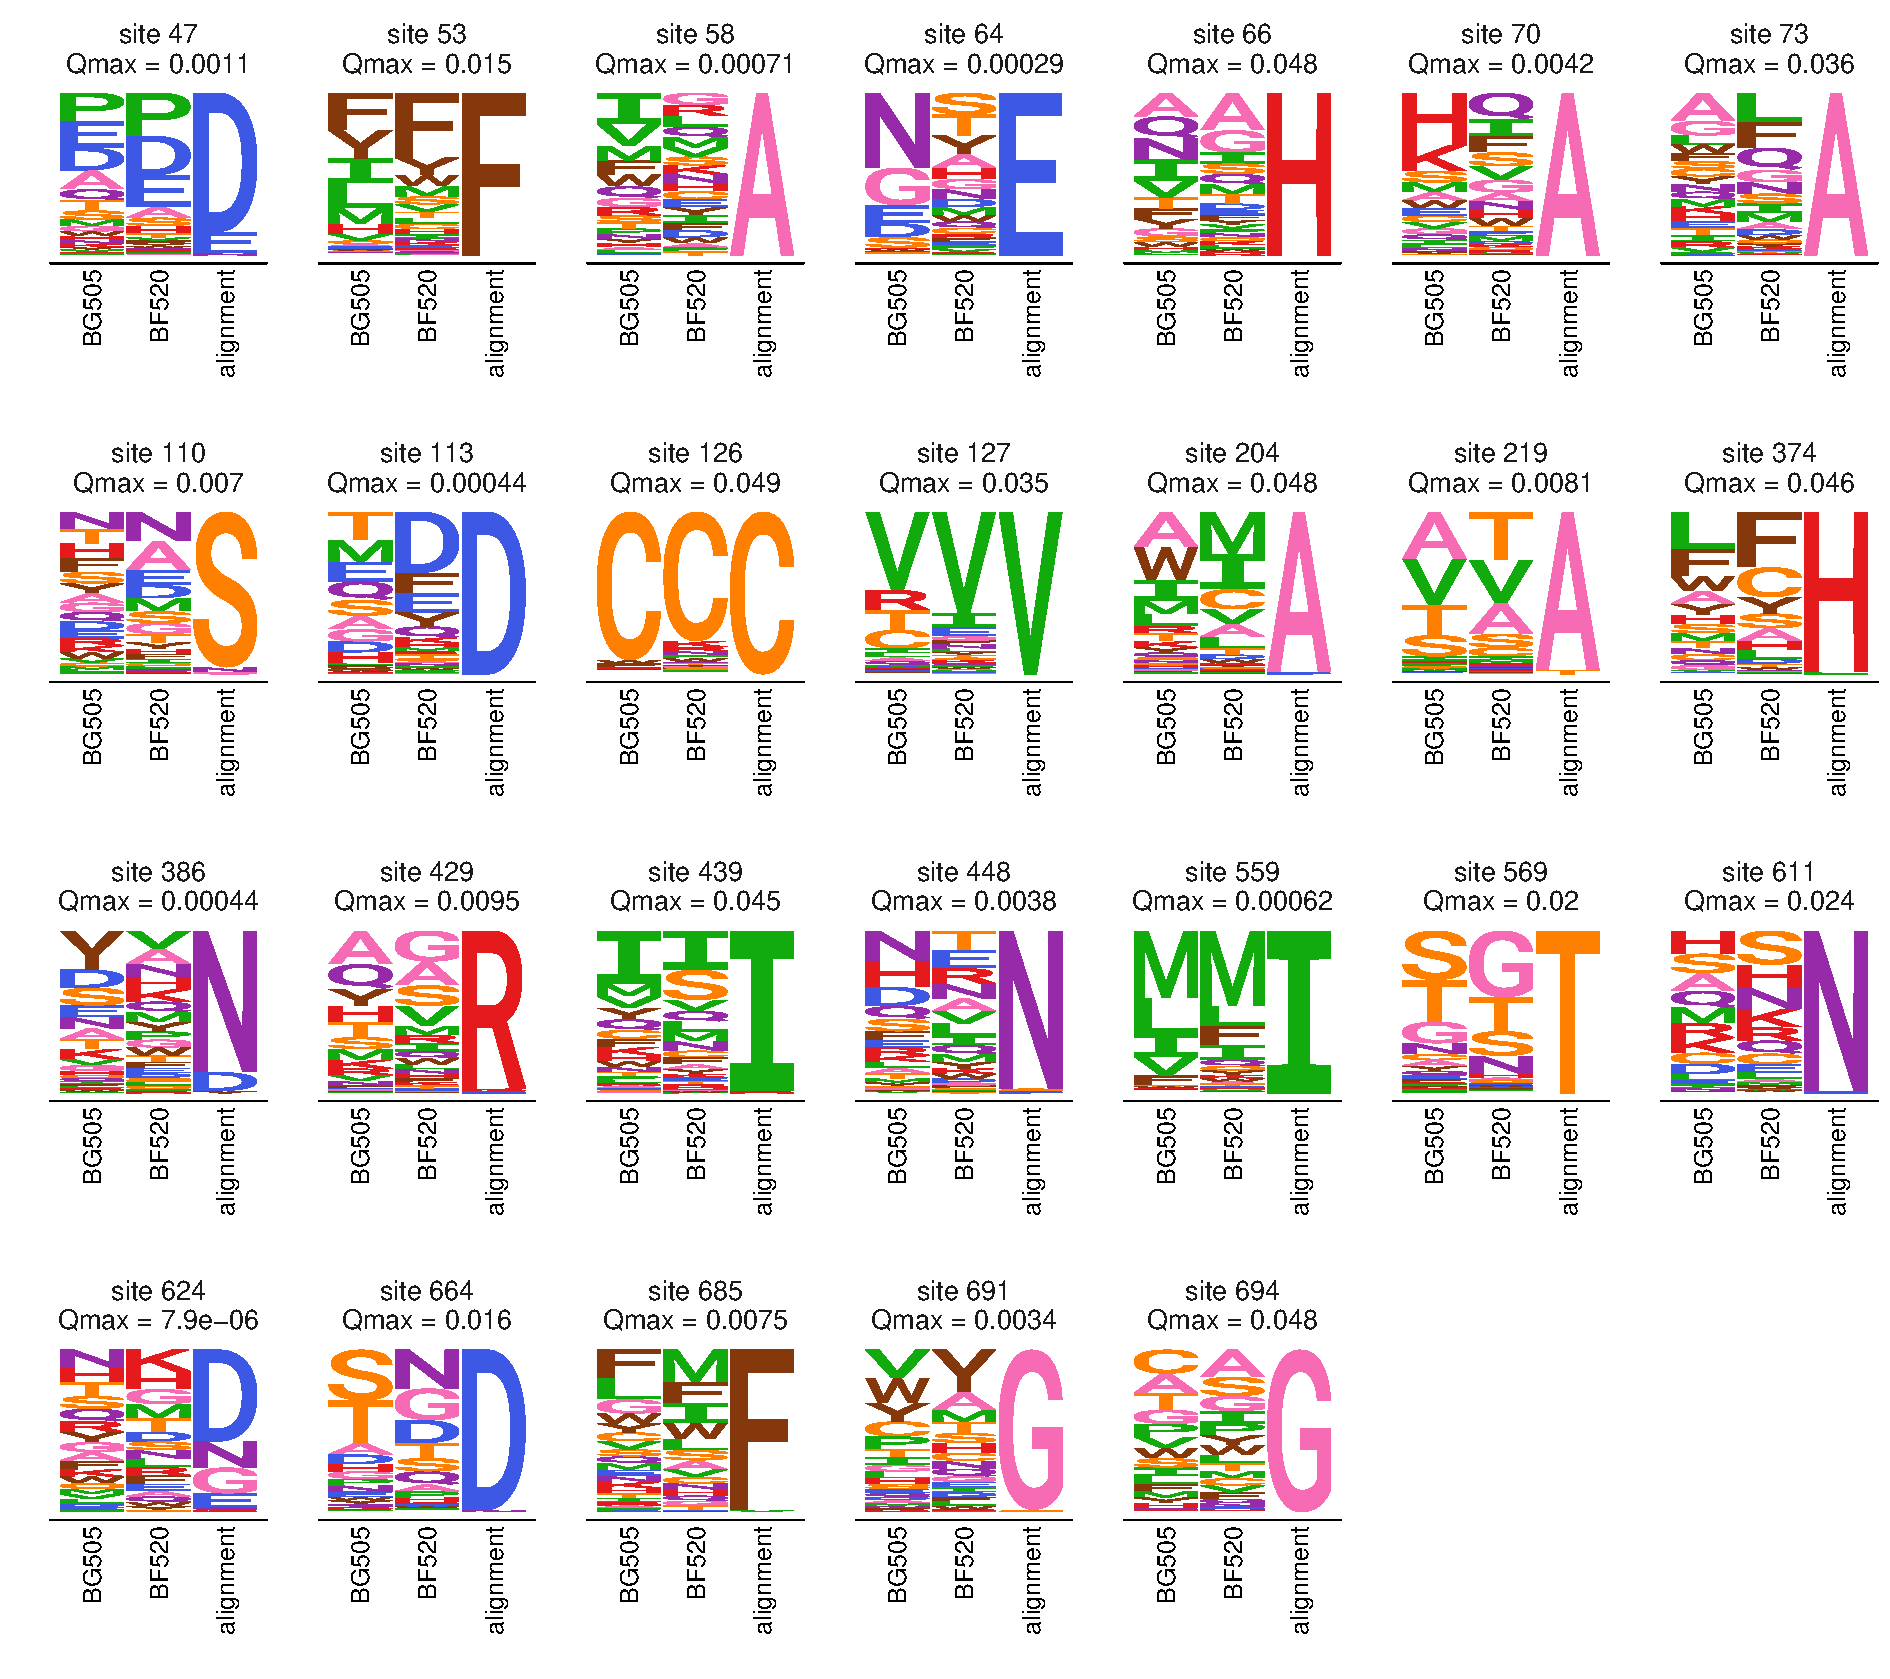
\includegraphics[width=\textwidth]{figures/purifying_selsites.pdf}}
\figsupp[Distribution of relative solvent accessibilities among sites of diversifying and purifying selection.]{
Sites are grouped by whether they are under diversifying or purifying selection at $Q < 0.05$ in \emph{both} homologs, or whether they do not fall into either of these categories.
The absolute solvent accessibility of each site in the BG505 SOSIP trimer in PDB 5FYL~\citep{?} was calculated using DSSP~\citep{?}, and normalized to a relative solvent accessibility using the absolute accessibilities provided by \citet{?}.
As can be seen from these box plots with overlaid points for each site, sites of both diversifying and purifying selection tend to have higher relative solvent accessibility than other sites.
}{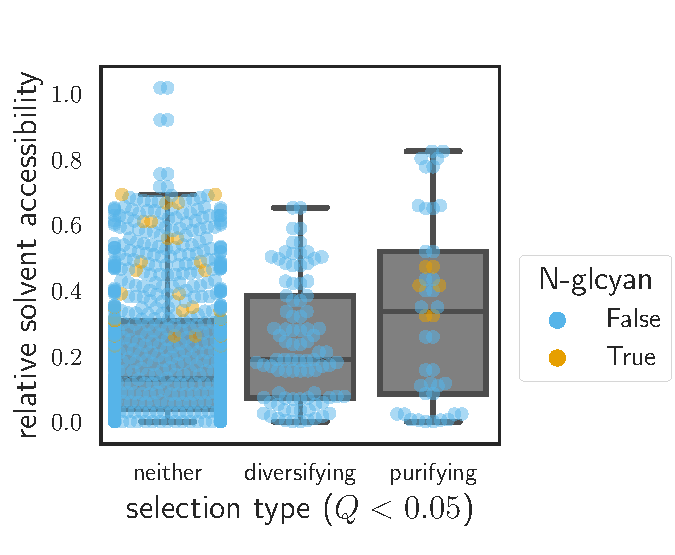
\includegraphics[width=0.5\textwidth]{figures/selsites_rsa.pdf}}
\figdata{The $\omega_r$ and associated $P$-values plotted in this figure are in \texttt{merged\_omegabysite.csv}.}
\end{figure}
\FloatBarrier


\subsection*{Differences between homologs}


\subsection*{Validating sites of mutational shifts}

\subsection*{Looking at how shifts relate to evolution and structure}


\section{Discussion}


\section{Methods and Materials}

\subsection*{Sequence alignments}

\section{Acknowledgments}

\bibliography{references.bib}

\begin{suppfile}
\caption{
\label{suppfile:code}
The code to perform all steps in the analysis beginning with downloading the FASTQ files is in \texttt{analysis\_code.zip}.}
\end{suppfile}


\end{document}
